
\section{АНАЛІЗ ПРЕДМЕТНОЇ ОБЛАСТІ СИСТЕМ МОНІТОРИНГУ РОЗВИТКУ НЕМОВЛЯТИ ТА ОГЛЯД ІСНУЮЧИХ РІШЕНЬ}

\subsection{Актуальність та доцільність розроблення}

За даними \gls{ВООЗ}, перші два роки життя дитини є найбільш інтенсивним періодом фізичного розвитку. Регулярний моніторинг маси тіла, зросту та окружності голови дозволяє педіатрам вчасно виявляти відхилення від вікових норм і призначати корекційні заходи на ранніх стадіях. Паралельно батьки щодня фіксують режим годування та сну, стан здоров'я, вакцинації та вікові досягнення -- дані, що формують повноцінну картину розвитку дитини і є незамінними під час лікарських консультацій.

Попри важливість систематичного ведення таких записів, більшість батьків і сьогодні покладаються на паперові щоденники або стандартні нотатки смартфона. Такий підхід має суттєві обмеження: дані легко втрачаються, їх неможливо автоматично перетворити на динамічні графіки, а ведення записів одночасно двома батьками з різних пристроїв призводить до неузгодженостей і втрати актуальності даних. Крім того, паперові записи не дозволяють зіставити показники дитини зі стандартними перцентильними кривими, що унеможливлює самостійну оцінку динаміки розвитку між лікарськими візитами.

У відповідь на ці потреби ринок мобільних застосунків для батьків активно розвивається. Проте, як показує аналіз наявних рішень, переважна більшість із них охоплює лише окремі аспекти моніторингу і не забезпечує комплексного підходу. Жоден із популярних застосунків не поєднує повноцінного антропометричного моніторингу відповідно до стандартів \gls{ВООЗ}, синхронізації між пристроями в реальному часі, що визначає практичну актуальність розроблення такої системи.

\subsection{Огляд та аналіз існуючих рішень}

На ринку мобільних застосунків для батьків існує декілька поширених рішень для відстеження розвитку немовляти. Їх функціональність варіюється від базового журналювання активностей до комплексного відстеження сну з аналітикою. Було розглянуто три найбільш популярних застосунки: Sprout Baby Tracker, Huckleberry та Glow Baby. Аналіз цих рішень дозволив виявити їхні ключові переваги та недоліки, а також визначити напрями для вдосконалення у розроблюваній системі.

\subsubsection{Sprout Baby Tracker}

Sprout Baby Tracker -- один із найстаріших і найвідоміших застосунків для відстеження немовляти, доступний на платформах iOS та Android. Застосунок орієнтований на ведення повноцінного журналу активностей дитини з перших днів життя і дозволяє фіксувати годування (грудне молоко та суміш), епізоди сну, зміни підгузників, вимірювання маси тіла та зросту, а також переглядати хронологію подій у вигляді стрічки. Передбачена підтримка декількох профілів дітей в одному обліковому записі, що зручно для сімей із двома і більше дітьми.

До переваг Sprout Baby Tracker належать зрілий і зручний інтерфейс, широка функціональність журналювання та надійна робота без підключення до мережі. Графіки зростання дозволяють відстежувати динаміку антропометричних показників, однак порівняння з перцентильними кривими \gls{ВООЗ} безпосередньо в застосунку відсутнє. Синхронізація між пристроями реалізована через хмарне резервне копіювання і не відбувається в реальному часі, що ускладнює спільне ведення записів двома батьками. 
\begin{center}
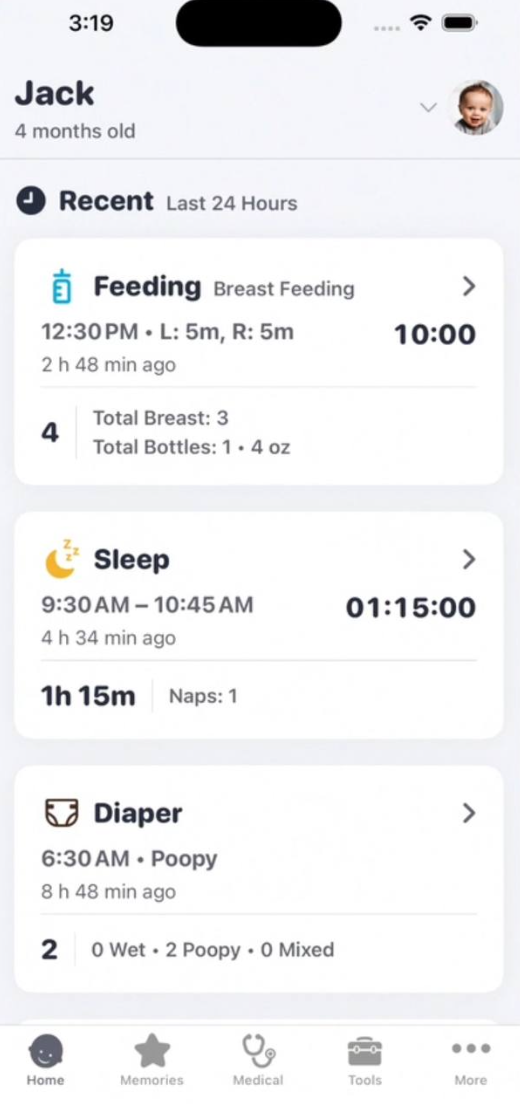
\includegraphics[height=0.45\textheight, keepaspectratio]{figures/sprout.jpg}
\captionof{figure}{Інтерфейс застосунку Sprout Baby Tracker}
\label{fig:sprout}
\end{center}

\subsubsection{Huckleberry}

Huckleberry -- застосунок, орієнтований передусім на аналіз сну немовляти. Його ключова функція -- алгоритм SweetSpot, який на основі накопичених даних про денний сон і нічний відпочинок пропонує оптимальний час для вкладання дитини. Застосунок збирає дані про тривалість і якість сну, фіксує годування та дозволяє вести загальні нотатки. Преміальна версія надає доступ до персоналізованих консультацій із сертифікованими фахівцями з дитячого сну.

Перевагою Huckleberry є глибока аналітика сну та наявність консультаційного сервісу, що виділяє його серед аналогів. Водночас застосунок має суттєві обмеження: повноцінний модуль антропометричного моніторингу з перцентильними кривими \gls{ВООЗ} відсутній, функціональність безкоштовної версії значно обмежена, а покрокового журналу активностей, який охоплював би всі аспекти догляду за немовлям, немає. 
\begin{center}
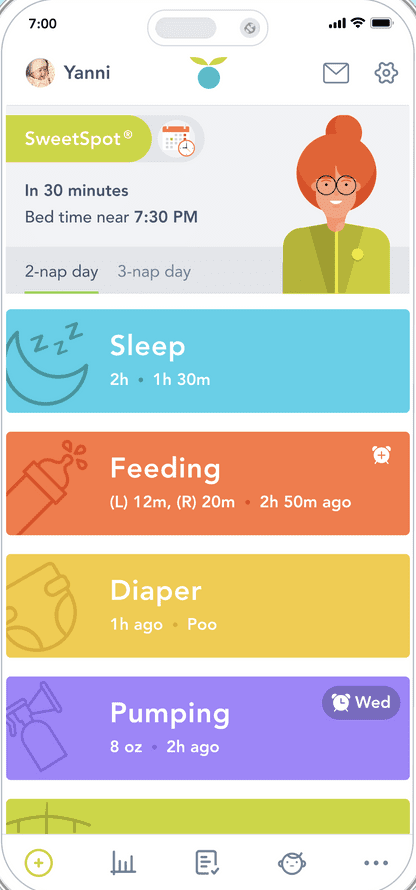
\includegraphics[height=0.45\textheight, keepaspectratio]{figures/huckleberry.png}
\captionof{figure}{Інтерфейс застосунку Huckleberry}
\label{fig:huckleberry}
\end{center}

\subsubsection{Glow Baby}

Glow Baby -- комплексний трекер розвитку дитини від компанії Glow Inc., доступний на iOS та Android. Застосунок охоплює журнал активностей (годування, сон, підгузники, купання), відстеження вікових досягнень за категоріями (моторика, мова, соціальний розвиток), базові графіки зростання та широку базу статей про догляд за немовлятами. Передбачена функція спільного доступу, що дозволяє обом батькам переглядати та додавати записи.

Glow Baby вирізняється широтою контенту, системою вікових підказок і наявністю спільного доступу для батьків. Проте порівняння антропометричних показників із перцентильними кривими \gls{ВООЗ} реалізоване спрощено і не відображає повний набір стандартів. Статті носять загальний інформаційний характер без прив'язки до конкретних даних дитини. Синхронізація між пристроями в режимі реального часу також не забезпечена.

\begin{center}
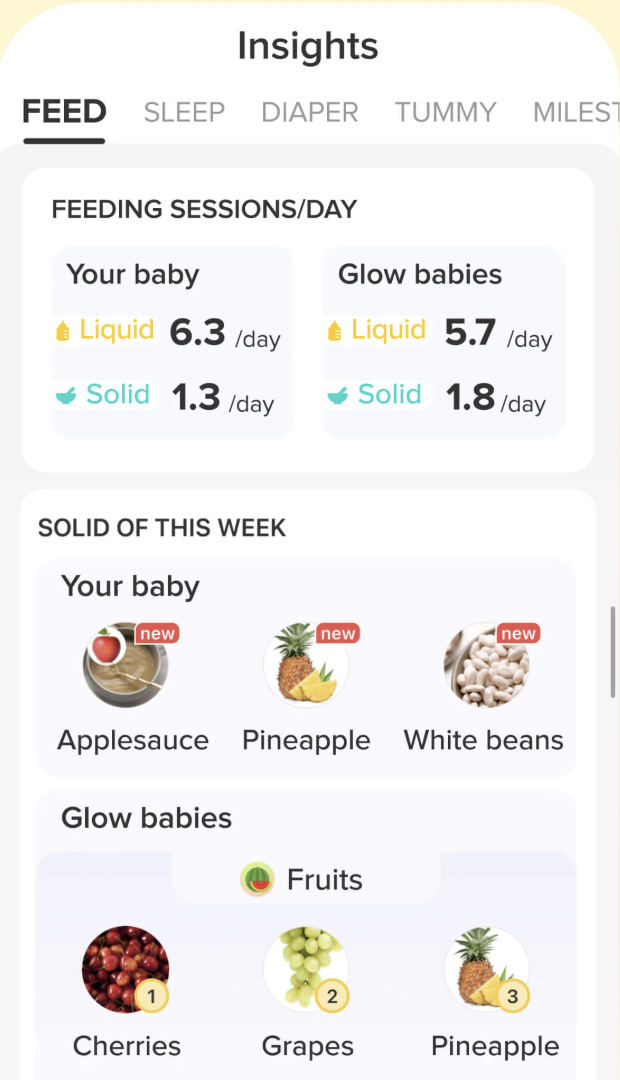
\includegraphics[height=0.55\textheight, keepaspectratio]{figures/glow.png}
\captionof{figure}{Інтерфейс застосунку Glow Baby}
\label{fig:glow}
\end{center}

\FloatBarrier
\subsection{Аналіз функціональності та вимог до системи}

\subsubsection{Порівняльна характеристика розглянутих рішень}

На основі огляду трьох застосунків проведено порівняльний аналіз їхніх ключових переваг і недоліків. Результати наведено в таблиці~\ref{tbl:comparison}.

\begin{table}[H]
\centering
\caption{Порівняльна характеристика існуючих рішень}
\label{tbl:comparison}
\begin{tabular}{|>{\raggedright\arraybackslash}p{3.0cm}|>{\raggedright\arraybackslash}p{6.2cm}|>{\raggedright\arraybackslash}p{6.2cm}|}
\hline
\textbf{Застосунок} & \textbf{Переваги} & \textbf{Недоліки} \\
\hline
\renewcommand{\baselinestretch}{1.5}\selectfont Sprout Baby Tracker &
\renewcommand{\baselinestretch}{1.5}\selectfont
1. Широкий журнал активностей \newline
2. Підтримка декількох профілів дітей \newline
3. Надійна робота без мережі
&
\renewcommand{\baselinestretch}{1.5}\selectfont
1. Відсутність кривих \gls{ВООЗ} \newline
2. Синхронізація не в реальному часі \\
\hline
\renewcommand{\baselinestretch}{1.5}\selectfont Huckleberry &
\renewcommand{\baselinestretch}{1.5}\selectfont
1. Глибока аналітика сну \newline
2. Алгоритм SweetSpot \newline
3. Чат з консультантом зі сну
&
\renewcommand{\baselinestretch}{1.5}\selectfont
1. Відсутність антропометричного модуля \newline
2. Обмежений безкоштовний функціонал \\
\hline
\renewcommand{\baselinestretch}{1.5}\selectfont Glow Baby &
\renewcommand{\baselinestretch}{1.5}\selectfont
1. Широкий контент та вікові підказки \newline
2. Спільний доступ для батьків \newline
3. База статей про догляд
&
\renewcommand{\baselinestretch}{1.5}\selectfont
1. Спрощені графіки без кривих \gls{ВООЗ} \newline
2. Загальні статті без прив'язки до даних \\
\hline
\end{tabular}
\end{table}

Проведений порівняльний аналіз демонструє, що кожна з розглянутих платформ має свої сильні сторони, але водночас і певні обмеження. Sprout Baby Tracker вирізняється зрілим інтерфейсом та широким журналом активностей, але не має підтримки кривих \gls{ВООЗ} та синхронізації в реальному часі. Huckleberry пропонує унікальну аналітику сну, проте є вузькоспеціалізованим і не забезпечує комплексного моніторингу. Glow Baby охоплює найширший спектр функцій серед аналогів, однак поступається у точності антропометричних графіків і не має персоналізованого \gls{ШІ}-асистента. Таким чином, жоден із розглянутих застосунків не поєднує повноцінного антропометричного моніторингу відповідно до стандартів \gls{ВООЗ} та синхронізації між пристроями в реальному часі, що обґрунтовує доцільність розроблення нового рішення.

Для наочного позиціонування розроблюваної системи відносно існуючих аналогів складено функціональну матрицю порівняння, наведену в таблиці~\ref{tbl:features}.

\begin{center}
\captionof{table}{Функціональна матриця порівняння застосунків}
\label{tbl:features}
{\small\renewcommand{\arraystretch}{1.15}
\begin{tabular}{|>{\raggedright\arraybackslash}p{4.8cm}|>{\centering\arraybackslash}p{2.4cm}|>{\centering\arraybackslash}p{2.2cm}|>{\centering\arraybackslash}p{2.1cm}|>{\centering\arraybackslash}p{2.6cm}|}
\hline
\textbf{Критерій} &
\textbf{Sprout Baby Tracker} &
\textbf{Huckleberry} &
\textbf{Glow Baby} &
\textbf{Розроблювана система} \\
\hline
Журнал активностей & Так & Частково & Так & Так \\
\hline
Антропометрія з кривими \gls{ВООЗ} & Ні & Ні & Частково & Так \\
\hline
Синхронізація в реальному часі & Ні & Ні & Ні & Так \\
\hline
Аналітика режиму сну & Ні & Так & Ні & Частково \\
\hline
Вакцинації та вікові досягнення & Частково & Ні & Частково & Так \\
\hline
Спільний доступ опікунів & Частково & Ні & Так & Так \\
\hline
\end{tabular}}
\end{center}

\subsubsection{Вимоги до реалізації застосунку}

З урахуванням аналізу існуючих рішень та потреб користувачів сформульовано функціональні та нефункціональні вимоги до розроблюваної системи. Вимоги формувалися з прагненням усунути виявлені недоліки аналогів і забезпечити комплексний інструмент для відстеження розвитку немовляти.

Функціональні вимоги:
\begin{enumerate}
  \item Реєстрація та автентифікація користувача через email і пароль із захищеним зберіганням сесії.
  \item Підтримка декількох профілів дітей та моделі опікунів: можливість запросити іншого користувача для спільного ведення записів.
  \item Ведення журналу активностей: годування (грудне молоко, суміш, прикорм), сон, підгузники, купання, температура, ліки.
  \item Додавання антропометричних вимірювань (маса тіла, зріст, окружність голови) та їх відображення на інтерактивних графіках із перцентильними кривими \gls{ВООЗ}.
  \item Управління графіком вакцинацій із відміткою виконаних щеплень.
  \item Відстеження вікових досягнень дитини з відміткою дати виконання.
  \item Синхронізація даних між пристроями в реальному часі через механізм підписки на зміни \gls{БД}.
\end{enumerate}

Нефункціональні вимоги:
\begin{enumerate}
  \item Кросплатформна підтримка iOS 16.0+ та Android 10+ із нативним відображенням компонентів інтерфейсу.
  \item Час відгуку \gls{API} не більше 500~мс для основних операцій при стабільному мережевому з'єднанні.
  \item Ізоляція даних між користувачами на рівні \gls{СУБД} засобами \gls{RLS}, незалежно від логіки клієнтського застосунку.
  \item Масштабованість хмарної інфраструктури для обслуговування зростаючої кількості користувачів без зміни архітектури.
  \item Захист застосунку від несанкціонованої модифікації та запуску на скомпрометованих пристроях.
\end{enumerate}

Визначені функціональні та нефункціональні вимоги є основою для проєктування архітектури системи та вибору технологічного стеку в наступних розділах.

\begin{conclusionsection}

\section{ВИСНОВОК ДО РОЗДІЛУ 1}

У першому розділі проведено аналіз предметної області: системи агрегації та обробки медико-біологічних даних немовляти в мобільному застосунку. Обґрунтовано актуальність розроблення: регулярний педіатричний моніторинг є критично важливим у перші два роки життя дитини, проте більшість батьків не має зручного цифрового інструменту для його ведення з підтримкою синхронізації між пристроями в реальному часі.

Здійснено огляд трьох популярних аналогів: Sprout Baby Tracker, Huckleberry та Glow Baby. Встановлено, що кожен із них орієнтований на певний аспект моніторингу: Sprout Baby Tracker охоплює широкий журнал активностей, Huckleberry спеціалізується на аналізі сну, а Glow Baby пропонує найбільший обсяг контенту серед аналогів. Водночас жоден із розглянутих застосунків не поєднує повноцінного антропометричного моніторингу з кривими \gls{ВООЗ} та синхронізації між пристроями в реальному часі.

На основі порівняльного аналізу сформульовано сім функціональних і п'ять нефункціональних вимог до розроблюваної системи. Функціональні вимоги охоплюють автентифікацію, модель опікунів, журнал активностей, антропометричний моніторинг із кривими \gls{ВООЗ}, вакцинації, досягнення та синхронізацію в реальному часі. Нефункціональні вимоги регламентують продуктивність, безпеку та масштабованість системи.

Визначені вимоги покладено в основу вибору технологічного стеку та проєктування архітектури системи, які розглядаються в наступних розділах.

\end{conclusionsection}
